%%%%%%%%%%%%%%%%%%%%%%%%%%%%%%%%%%%%%%%%%%%%%%%%%%%%%%%%%%%%%%%%%%%%%%%%%%%%%%%%
%2345678901234567890123456789012345678901234567890123456789012345678901234567890
%        1         2         3         4         5         6         7         8

%\documentclass[letterpaper, 10 pt, conference]{ieeeconf}  % Comment this line out
                                                           % if you need a4paper
\documentclass[a4paper, 10pt, conference]{ieeeconf}        % Use this line for a4
                                                           % paper

%\IEEEoverridecommandlockouts                               % This command is only
                                                           % needed if you want to
                                                           % use the \thanks command
\overrideIEEEmargins
% See the \addtolength command later in the file to balance the column lengths
% on the last page of the document



% The following packages can be found on http:\\www.ctan.org
\usepackage{graphics} % for pdf, bitmapped graphics files
\usepackage{epsfig} % for postscript graphics files
\usepackage{subfigure} % ben: is this package allowed?
%\usepackage{mathptmx} % assumes new font selection scheme installed
%\usepackage{times} % assumes new font selection scheme installed
%\usepackage{amsmath} % assumes amsmath package installed
%\usepackage{amssymb}  % assumes amsmath package installed

\title{\LARGE \bf
On Physics-Based 3D Waypoint Generation for Autonomous Exploration in Aerial Robotics
}

\iffalse
\author{ \parbox{3 in}{\centering Benjamin Adler\\
         Fachbereich Informatik, Technische Aspekte Multimodaler Systeme (TAMS)\\
         University of Hamburg\\
         Hamburg, Germany\\
         {\tt\small adler@informatik.uni-hamburg.de}}
         \hspace*{ 0.5 in}
         \parbox{3 in}{ \centering Jianwei Zhang\\
         Fachbereich Informatik, Technische Aspekte Multimodaler Systeme (TAMS)\\
         University of Hamburg\\
         Hamburg, Germany\\
         {\tt\small zhang@informatik.uni-hamburg.de}}
}
\fi

\author{Benjamin Adler and Jianwei Zhang\\
        University of Hamburg\\
        Fachbereich Informatik,\\
        Technische Aspekte Multimodaler Systeme (TAMS)\\
        Hamburg, Germany\\
        {\tt\small adler@informatik.uni-hamburg.de}%
}

\begin{document}



\maketitle
\thispagestyle{empty}
\pagestyle{empty}


%%%%%%%%%%%%%%%%%%%%%%%%%%%%%%%%%%%%%%%%%%%%%%%%%%%%%%%%%%%%%%%%%%%%%%%%%%%%%%%%

\begin{abstract}

This paper presents a novel, physics-based approach to computing waypoints, which are subsequently being used to steer a flying platform in three-dimensional space to map an outdoor environment. Because the algorithm relies on simple physical processes, it is both easy to understand and implement in combination with traditional data structures. Generation of efficient sensor trajectories for maximized information gain operates directly on unorganized point clouds, creating a perfect fit for environment mapping with commonly user LIDAR sensors or time-of-flight cameras. We also present the algorithm by simulating its performance in a virtual outdoor scenario.

\end{abstract}

%%%%%%%%%%%%%%%%%%%%%%%%%%%%%%%%%%%%%%%%%%%%%%%%%%%%%%%%%%%%%%%%%%%%%%%%%%%%%%%%


\section{Introduction}

Automatic model building has always been one of the most important parts of autonomous robotics. Exploration and mapping - as a subclass of this problem - has been the topic of many papers in recent years. The SLAM problem was first solved for two-dimensional mapping scenarios and later-on expanded to three-dimensional environments.% \cite{shen2011}.

This paper presents a novel approach on increasing the efficiency of such mapping procedures. While the implementations of SLAM have improved greatly in recent years, one aspect of mapping three-dimensional environments was given comparatively little attention: finding the next best view. Typically, SLAM algorithms have been researched and developed on mobile platforms moving on flat surfaces \cite{walthelm2011}, \cite{yamauchi1998}, \cite{joho2007}. This setup does not require a high efficiency in exploration, as it does not inherently impose time constraints. The authors of this paper, however, are implementing exploration and mapping algorithms on a flying platform with a maximum flight time of less than 15 minutes. Aiming to explore as much of the environment as possible within this limited time motivates an efficient way of finding sensor poses (and in extension, sensor trajectories) that enable sensors to deliver as much information as quickly as possible. While repeatedly passing over the unknown environment in scan-line fashion results in very fast scanning, a better approach needs to be found to ensure scanning of surfaces that are shadowed from those sensor trajectories.

This paper is organized as follows: the next section investigates other authors work of recent years in this and related fields. In the subsequent chapters, we first introduce the hardware platform used for testing our implementations and then advance to explaining the basic datastructures our algorithm relies on. After our algorithm is explained and illustrated, we discuss its computational complexity and the results achieved so far. In the final chapter, we share our thoughts on its current limitations and future developments.

\section{Related Work}

Since the introduction of SLAM, much work has been done to refine and extend the algorithm for use in both two- and threedimensional environments. Finding the next best view, though, has never been a part of the SLAM problem \cite{gonzalez_banos2002} and is thus rarely addressed by these works.

Generating safely reachable waypoints from previously acquired sensor data is an extension of next-best-view problem (which itself is an extension to the art-gallery problem \cite{orourke1987}), as it does not include the constraints of safe navigation and instead deals with the generation of isolated viewpoints\cite{chen2008}. As sensor poses in areas between known and unknown environment offer a good compromise between safe reachability and high information gain, frontier-based approaches are a popular method to compute new waypoints in two-dimensional space and are well documented in the literature \cite{gonzalez_banos2002}, \cite{strand2009}, \cite{yamauchi1998}, \cite{shade2011}. Unfortunately, information about exploration boundaries is hard to generate from three-dimensional pointclouds.

As our robot is very maneuverable, the generated waypoints and trajectories can be created with less concern of the platform's ability to catenate them due to motion constraints that other tyes of vehicles (e.g. fixed-wing UAVs) previously entailed \cite{hota2009}. The common problem of wind, manifesting as both opportunity and hindrance, but mostly in the form of further constraints on feasible paths for many UAVs has spawned many contributions in the past \cite{mcgee2005}, \cite{mcneely2007}. Even though wind is still a matter of concern for our platform, it does no longer influence the design of path planning or waypoint generation, but only localization and motion control.

\section{Our approach}

\subsection{Platform}

\begin{figure}[thpb]
  \centering
  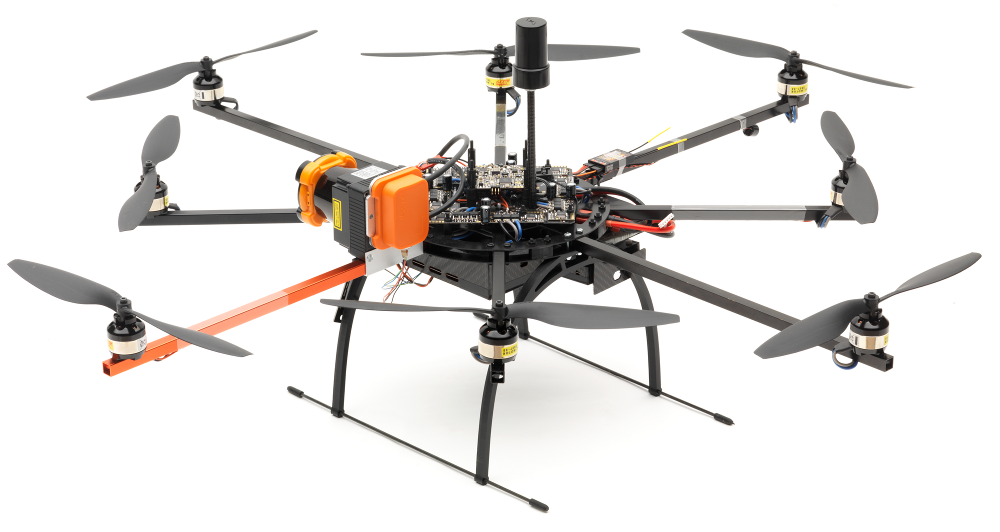
\includegraphics[width=0.5\textwidth]{images/oktokopter_photo_small}
  \caption{The experimental flying platform with mounted GNSS-antenna/receiver, processor-board, laser scanner and IMU.}
  \label{oktorendering}
\end{figure}

%\cite{mikrokopterproject}
To save time during the construction of our platform, we used an ``Okto 2''-octocopter from the mikrokopter-project as a base for our vehicle (see Fig. \ref{oktorendering}). Its central FlightControl (FC) processor-board is connected to eight brushless-motor controllers (BL) via an $I{^2}C$ bus. Employing its on-board gyros and accelerometers, the FC is programmed to stabilize the platform by itself when no other motion-control-commands are received from either the connected remote-control-receiver or the serial port. The project also developed the NaviControl (NC), an add-on hardware module that sends motion-control-commands (thrust, yaw, pitch and roll each as 8-bit signed integers) to steer the platform to waypoints. We abandoned the idea of using the NC for our purposes, as its hardware adds extra weight and its control-algorithms are neither capable of moving the platform as desired nor open-source. Instead, we fitted an Intel Atom processor-board to the platform. This board has a serial connection to the FC, which is used to send motion-control-commands and receive sensor input.

\begin{figure}[b]
  \centering
  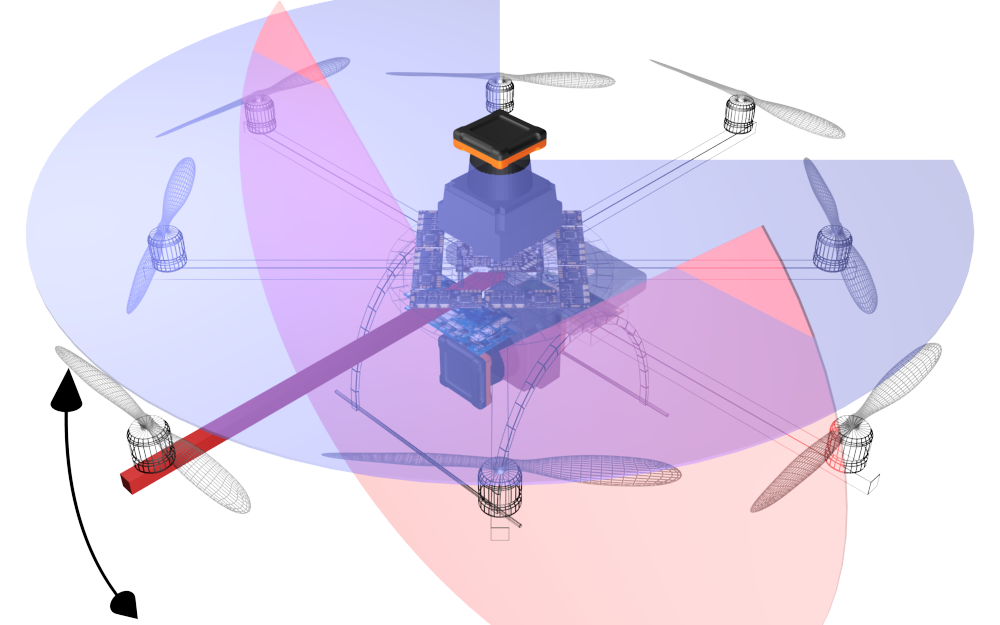
\includegraphics[width=0.44\textwidth]{images/scannerpair}
  \caption{Setup using two scanners with collision avoidance requiring permanent pitching motion}
  \label{lidar_setup_pair}
\end{figure}

A Septentrio AsterX2i RTK-GNSS (Real Time Kinematic Global Navigation Satellite System) receiver has been installed and connected to an XSens MTi IMU, enabling measurement of the platform's pose at 20Hz. Due to RTK-GPS, the position is accurate to within 5cm while the orientation shows a maximum error of $\sim1^\circ$ for pitch and roll and $\sim3^\circ$ for yaw angles. To shield the GNSS-receiver from electrostatic interferences caused by the processor board and protect from physical damage, both have been encapsulated into electrically shielded carbon-fiber boxes.

%Early positioning tests have shown promising results in open spaces. In more crowded areas, where multipath reception becomes a potential problem IR-anti-multipath

The laser scanner (Hokuyo UTM 30 LX) rotates at 2400rpm and provides both falling and rising edges after each complete scan of its 270$^\circ$ field of view. This signal is connected to the GNSS receiver, which is configured to emit the GPS Time Of Week (TOW) of the event with microsecond-precision on its USB-connection to the Atom processor-board. With both poses and laser scanner events being timestamped by the GNSS-receiver's time system, we can interpolate the vehicle's pose to the scanner's pose at the time of each scan.

\begin{figure}[b]
  \centering
  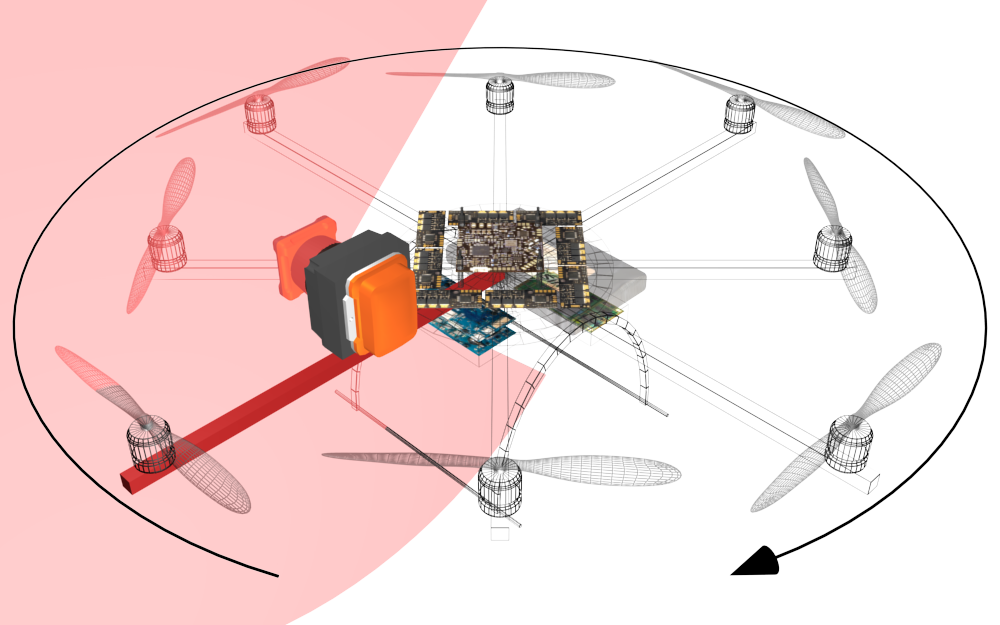
\includegraphics[width=0.44\textwidth]{images/scannersingle}
  \caption{Setup using single scanner, requiring permanent yawing motion}
  \label{lidar_setup_single}
\end{figure}

We initially planned to use two laser scanners, one with its scan-plane perpendicular to both the platform's groundplane and its forward-vector for scanning the environment and another scanner oriented to have its scan-plane parallel to the vehicle's ground-plane for collision-avoidance (see Fig. \ref{lidar_setup_pair}). Besides the obvious disadvantages of another 250 grams of payload and $\sim$10W of power consumption, the platform would have had to constantly pitch during flight to ensure reliable obstacle scanning and detection. Superimposing the pitching motion has proven to result in considerable amounts of work for the motors on the platform's front and back, reducing flight time. The non-constant angular pitching speed in this setup also necessitates a more precise interpolation of the vehicle's to the scanner's pose.

To avoid these drawbacks, we instead mounted a single laser scanner as depicted in Fig. \ref{lidar_setup_single}. By permanently yawing the platform in-flight, a single scanner captures both geometry for surface reconstruction and collision avoidance, provided that the world is static and the platform does not move further than the laser scanners' range within one rotation. Given a constant angular yawing-speed, the disadvantage of precise interpolation of the platform's pose becomes less problematic.
% TODO: speed < lidar-range * drehgeschwindigkeit ?

After balancing the platform's extra loads, it exhibits very favorable flight dynamics and drifts very slowly when idling. A switch on the remote control can be used to toggle between remote-control and computer-control. In the latter mode, the engines thrust will never exceed the value set on the remote control, providing ideal conditions for testing motion controllers. Including payload and a 5000mAh 4s1p LiPo battery, the platform weighs 2250 grams and requires around 350W of power while hovering, leading to a flight-time of up to 12 minutes.

%TODO \subsection{Motion Control}? Ausrichtung zum Ziel, konstantes drehen?

\subsection{Data structures}

Occupancy grid maps - and in extension elevation maps - are often used to store sensor data in generalized form \cite{shade2011}. Although the data structure permits easy traversability computation and frontier detection, storing more complex geometry or overhangs remains difficult or even impossible, limiting its practical use to two-dimensional environments. Furthermore, its uniform grid size requires a global compromise between model quality and memory consumption. Multi-Level surface maps, introduced by Triebel et al. \cite{triebel2006}, eliminate many of these limitations, while still being constrained to a grid.

%\cite{meagher1982}
In order to capture sensor data representing arbitrarily complex geometry and detail, we decided to implement our algorithm on an octree-based data-structure. Octrees are well suited for storing information in non-uniform resolution and the process of storing and retrieving data can easily be executed in parallel, allowing for optimization of parts of our algorithms. Besides its position, each point in the octree also stores its brightness (i.e. intensity as measured by the laser scanner) and a vector pointing from that point back to the sensor. As the platform's measured orientation is less precise that its measured position, this vector's length will be used lateron to assign points recorded from further distance (and thus suffering a greater impact from platform-orientation errors) a lesser weight in the following surface reconstruction.

%\begin{figure}[ht]
%  \centering
%  \subfigure[Initial setup]{
%    \label{process_1}
%    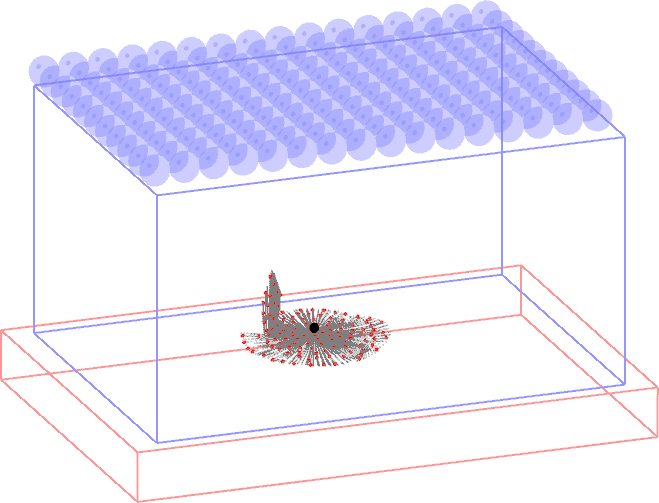
\includegraphics[width=0.4\textwidth]{images/process_side/1}
%  }
%  \subfigure[Physics simulation]{
%    \label{process_2}
%    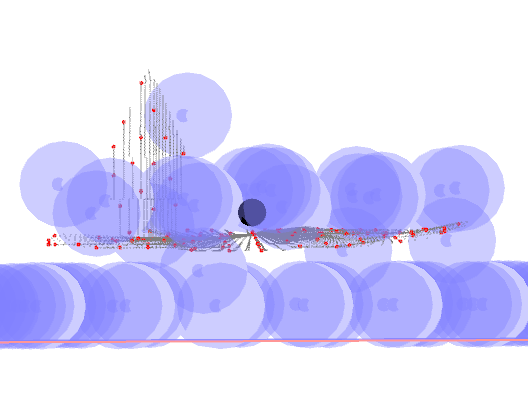
\includegraphics[width=0.4\textwidth]{images/process_side/2}
%  }
%  \subfigure[Waypoints and residual sampling geometry]{
%    \label{process_3}
%    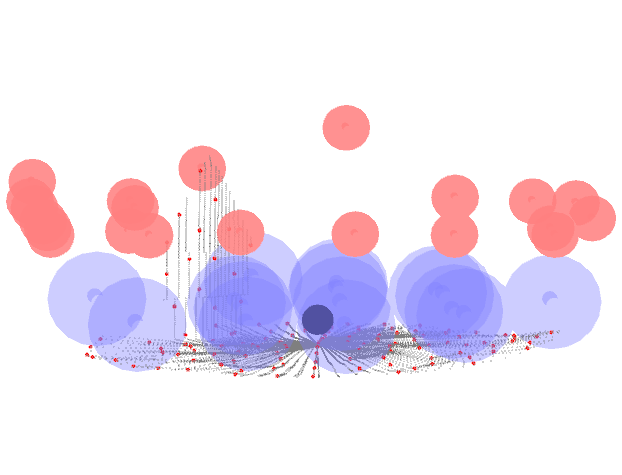
\includegraphics[width=0.4\textwidth]{images/process_side/3}
%  }
%  \subfigure[Generated waypoints]{
%    \label{process_4}
%    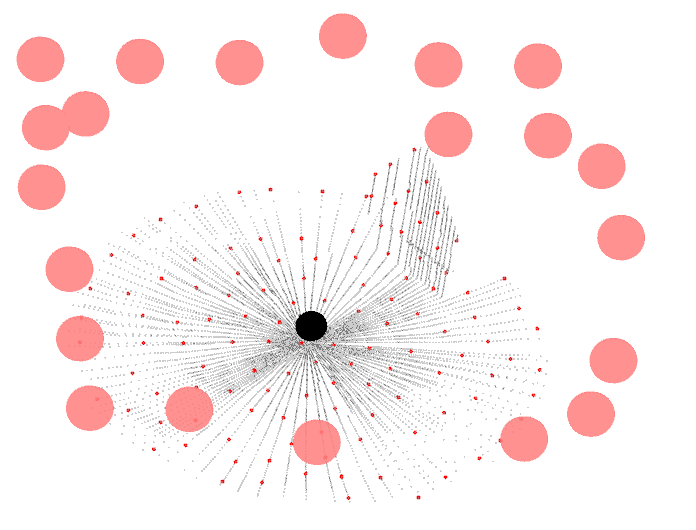
\includegraphics[width=0.4\textwidth]{images/process_side/4}
%  }
%  \caption{Waypoint generation, orthogonal projection; the bounding volume is blue, detection volume is red, vehicle position is black, pointcloud for geometry reconstruction is grey and pointcloud for waypoint generation is red. Second figure shows sampling geometry interacting with pointcloud. Geometry hitting the red volume will be converted to a waypoint at the position it last hit a point from the pointcloud. The last figure shows generated waypoints in red for an initial pointcloud population.}
%  \label{explanation_of_process}
%\end{figure}

\subsection{Algorithm}

\begin{figure*}[htb]
  \centering
  \subfigure[]{
    \label{method_1}
    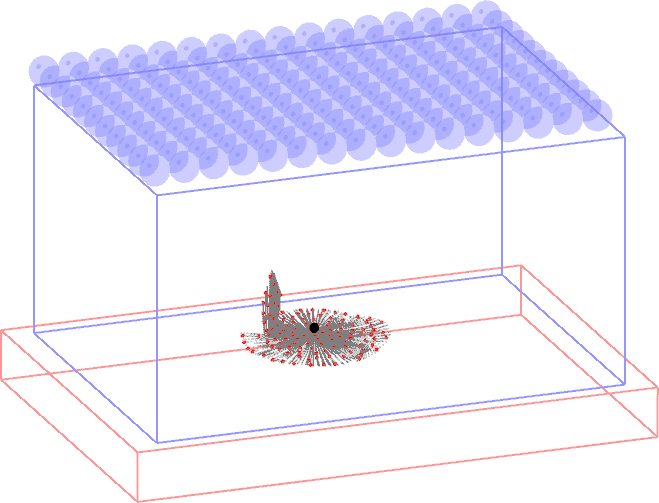
\includegraphics[width=0.43\textwidth]{images/process_side/1}
  }\hfill
  \subfigure[]{
    \label{method_2}
    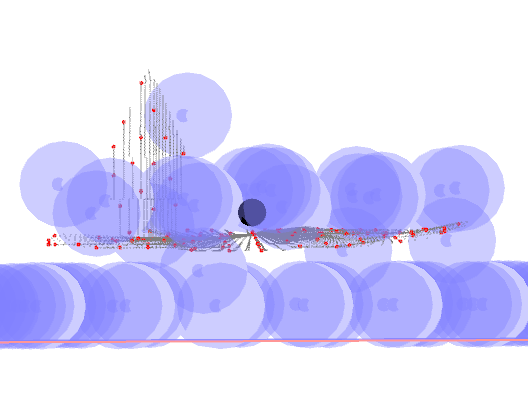
\includegraphics[width=0.43\textwidth]{images/process_side/2}
  }
  \subfigure[]{
    \label{method_3}
    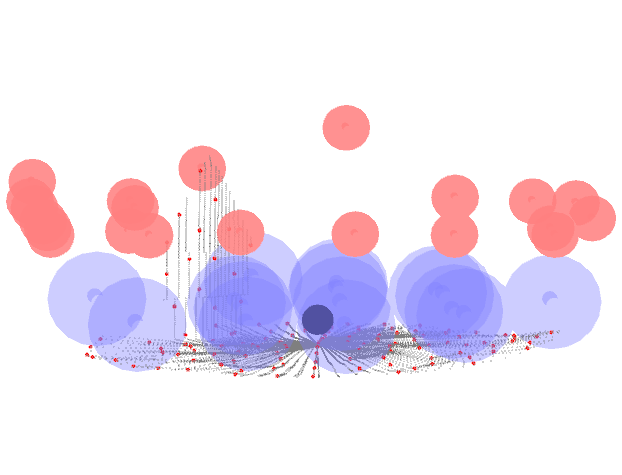
\includegraphics[width=0.43\textwidth]{images/process_side/3}
  }\hfill
  \subfigure[]{
    \label{method_4}
    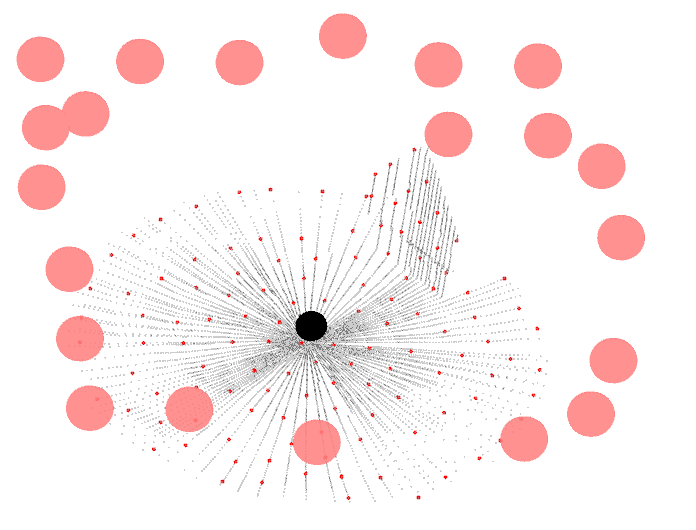
\includegraphics[width=0.43\textwidth]{images/process_side/4}
  }
  \caption{Waypoint generation, orthogonal projection; a) depicts the initial setup: the bounding volume is blue, detection volume is red, vehicle position is black, pointcloud for geometry reconstruction is grey and pointcloud for waypoint generation is red. b) shows sampling geometry interacting with pointcloud. In c), geometry hitting the red volume below is converted to a waypoint. The last figure d) shows generated waypoints in red for an initial pointcloud population. Please see http://tinyurl.com/physwpt for an animation of the process.}
  \label{explanation_of_process}
\end{figure*}

Three-dimensional environment mapping is often implemented using laser scanners and time-of-flight cameras, so unorganized point clouds are a very common type of sensor data. Any sensor generating spatial occupancy information can be used with our algorithm, as the pointcloud is its only sensory input. Finding the next best view in such data can be very hard, as it does not supply any information about geometric structures such as corners, edges, surfaces and normals. In contrast to many other algorithms (\cite{joho2007}, \cite{walthelm2011}), ours does not require such information.

Prior to the mapping process, the user creates a bounding volume as a representation of the region-of-interest around the vehicle's starting position, thereby defining the environment that is to be mapped. All generated viewpoints will be constrained to this volume and its vicinity, ensuring that the vehicle does not leave the scene. During initialization, a physics engine is set up with a detection volume below the defined bounding volume. Each new point in the pointcloud is automatically registered as a collision object in the physics world. After the octree is populated with an initial set of points (i.e. right after lift-off), the waypoint generation algorithm is executed as depicted in Fig. \ref{explanation_of_process}:

\begin{enumerate}
     \item Create and initialize sample geometry: spheres of user-defined size are spwaned evenly along the bounding volume's top plane. Increasing the sample geometry's size will create fewer instances, less computational burden (see section \ref{complexity}) and less waypoints, while decreasing the size will find smaller holes the the sampled surface.
     \item Start the physics simulation, allowing the sampling geometry to follow the defined gravity. Whenever a sample geometry instance collides with a point registered in the pointcloud, that event is saved into a special data structure mapping every sample geometry instance to its position in that moment. As this data structure is implemented as a map, later events caused by the same sampling geometry instance replace its previously saved position.
     \item When a sample geometry instance collides with the detection volume, it is removed from the simulation and the position of its last collision on the ground-plane is recorded as a waypoint marker.
     \item Waypoint markers are converted to waypoints if there are no other waypoints in close vicinity. When converting markers to waypoints, their height needs to be adjusted, as waypoint markers tend to spawn on the scenery's ground. The distance $d$, by which markers are lifted before becoming waypoints, is calculated by $d = Range_{lidar} * \frac{SizeSampleGeom_{current}}{SizeSampleGeom_{max}}$. By making the distance from laser scanner to the scanned surface depend on the size of the surface's holes, a natural behavior emerges: The vehicle will first scan larger voids in the surface from further away, then, as the sampling geometry's size is reduced in later iterations of the waypoint generation, come closer to fill smaller defects that couldn't be seen from former sensor poses.
\end{enumerate}

Physics simulation stops when all sampling geometry has either been deleted after hitting the delection volume, is currently in sleep state or has stopped moving entirely. Depending on the solver employed in the physics calculations, the weight of the involved bodies and the number of contact pairs between them, the latter criterion cannot always be fulfilled, as numerical instabilities can cause simulated objects to continue moving indefinetely. For this reason, we implemented a threshold-based approach, putting slowly-moving bodies in sleep states until they are reactivated by impulses from other bodies. This way, termination of the physics computation is guaranteed.

% \cite{sun2002}, 
Depending on size, number and shape of sampling geometry, this method simulates exposing the scanned surface to a fluid pushing through the model. The idea of generating watertight models from previously generated datasets is rather common and already well researched \cite{hornung2006}, \cite{sormann2007}, so the novelties here are:


\begin{itemize}
 \item testing the currently collected data for watertightness in-flight and using the result as a termination criterion for exploration.
 \item testing for watertightness using a physical simulation and its real-time implementation directly on sensor-data without additional pre-processing.
 \item compromise between exploration time and quality of resulting model can be changed quickly and in-flight by changing sampling geometry size.
 \item the algorithm's gracefully degraded behavior when size and number of sampling geometry cannot be scaled to achieve simulation with near-fluid behavior due to constrained computational resources.
\end{itemize}

Although any geometry can be used for waypoint generation, using spheres yields three important advantages:

\begin{itemize}
  \item Spheres can be represented only by radius and position, reducing the overall memory requirement (especially when all spheres share a common radius).
  \item Collision detection between points and spheres is a process of low computational complexity, even redundantizing the midphase in collision detection. To detect a collision, it is sufficient to check whether the distance between the sphere's center and the point is smaller than the sphere's radius.
  \item Most importantly, spheres are ideally suited to slip through smaller ``holes'' in the pointcloud, enabling their detection.
\end{itemize}

\begin{figure*}[htb]
  \centering
  \subfigure[]{
    \label{process_1}
    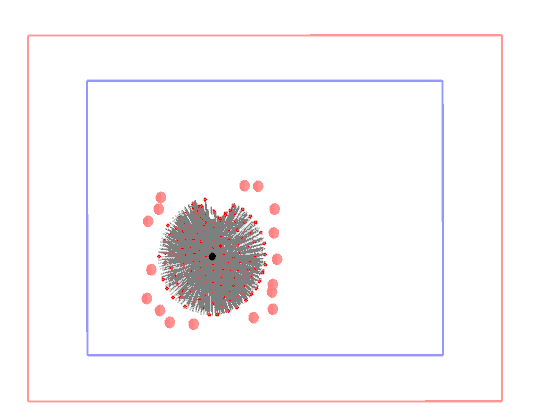
\includegraphics[width=0.3\textwidth]{images/process_top/1}
  }
  \subfigure[]{
    \label{process_2}
    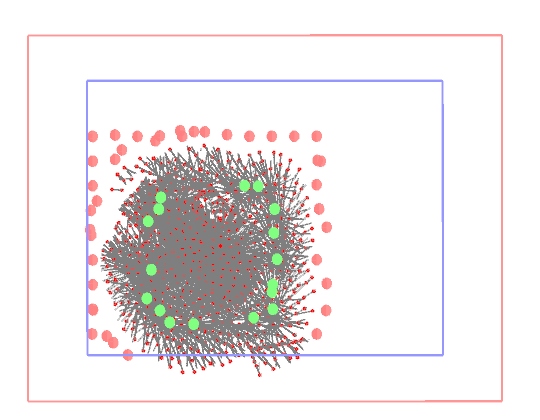
\includegraphics[width=0.3\textwidth]{images/process_top/2}
  }
  \subfigure[]{
    \label{process_3}
    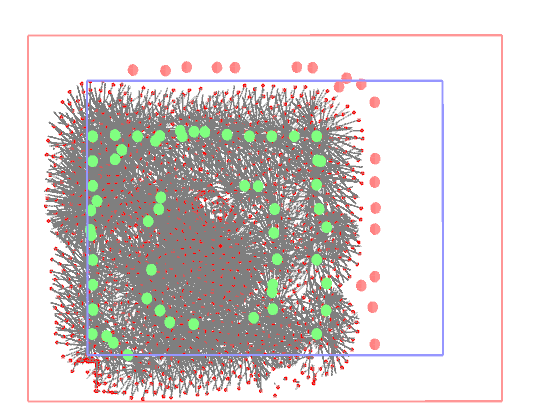
\includegraphics[width=0.3\textwidth]{images/process_top/3}
  }
  \subfigure[]{
    \label{process_4}
    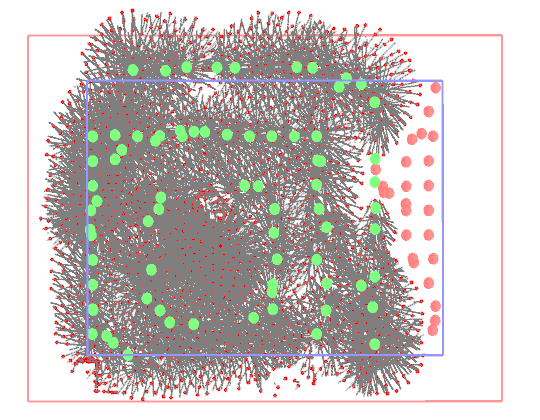
\includegraphics[width=0.3\textwidth]{images/process_top/4}
  }
  \subfigure[]{
    \label{process_5}
    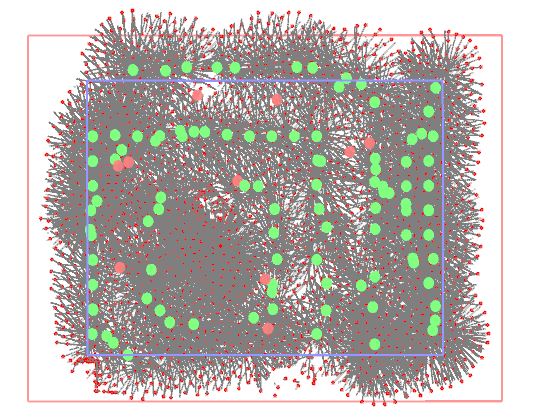
\includegraphics[width=0.3\textwidth]{images/process_top/5}
  }
  \subfigure[]{
    \label{process_6}
    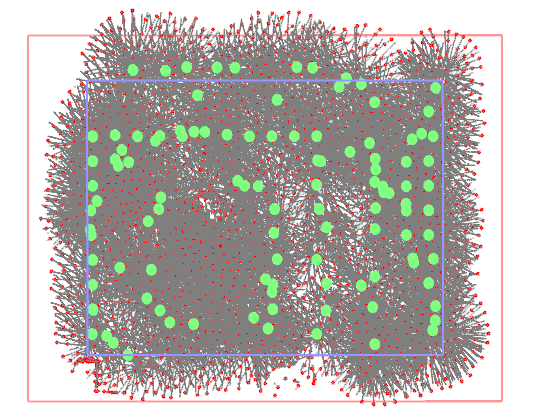
\includegraphics[width=0.3\textwidth]{images/process_top/6}
  }
  \caption{As seen from the top, multiple iterations of waypoint generation lead to continuous scanning at the border between known and unknown environment. Red waypoints are enqueued for scanning, green waypoints have been passed. In figures a) to d), sample spheres with $r=3m$ have been used to quickly explore the landscape, while in figure e), sampling geometry of reduced size ($r=1.5m$) has allowed finding smaller holes in previously scanned surfaces.}
  \label{figure_process}
\end{figure*}


%\subsection{Information Gain}
%To increase the sampled area of 
%weil die kugeln, die von der kante fallen, (am meisten) z�hlen, bekomme ich immer wegpunkte mit dem gr��ten information gain?!

\subsection{Computational complexity}
\label{complexity}

The algorithms complexity derives from the computational effort of the collision detection phase in physics simulation and thus from the number of collision objects. Collision detection between $n$ objects in general requires $n(n-1)/2$ collision checks to be performed, leading to a complexity of O($n^2$). Optimized algorithms like sort-and-sweep (\cite{baraff1992}) or implementations relying on spatial subdivison may reduce the complexity to O($n$ log $n$) in favorable cases \cite{legrand2007}. This initially appears to be a major obstacle to employment of the algorithm outside of simulation, as the pointcloud may grow to several million points during a scan; after the following optimizations, however, the algorithm has proven to be sufficiently fast for real-time application on current-generation CPUs.

\begin{itemize}
  \item Given a pointcloud consisting of $n$ points and a set of $m$ sample geometries, the algorithm does not require collision tests between all $n+m$ objects. As the $n$ points making up the accumulated scan data are static, the number of required tests is reduced to $\frac{m(m-1)}{2} + n*m$. Because $n \gg m$, this optimization yields a considerable loss in computational effort.

  \item When using the sensordata solely for waypoint generation, the density of the pointcloud can be reduced to allow gaps almost the size of the sample geometries' radius. That is, if sample spheres are created with a radius of e.g. $r = 1m$, the octree storing that pointcloud may discard points if there are neighbors within a distance of less than $2r$. This is implemented by simple neighbor-queries during insertion of candidate points and - while causing a higher computational complexity in that phase - yields a reduction of $n$ by about two dimensions, dramatically reducing the number of collision pairs that have to be checked in every step of the physics simulation. For this reason, we use two pointclouds in our work; one is used for surface reconstruction and is stored in an octree which allows for close neighbors (and thus high density) and another pointcloud used for waypoint generation and collision avoidance.

  \item As described in Le Grand's work \cite{legrand2007}, execution of the simulation's broadphase on GPU can speed up collision detection by more than an order of magnitude compared to calculation on the CPU.
\end{itemize}

\section{Results}

\begin{figure}[bt]
  \centering
    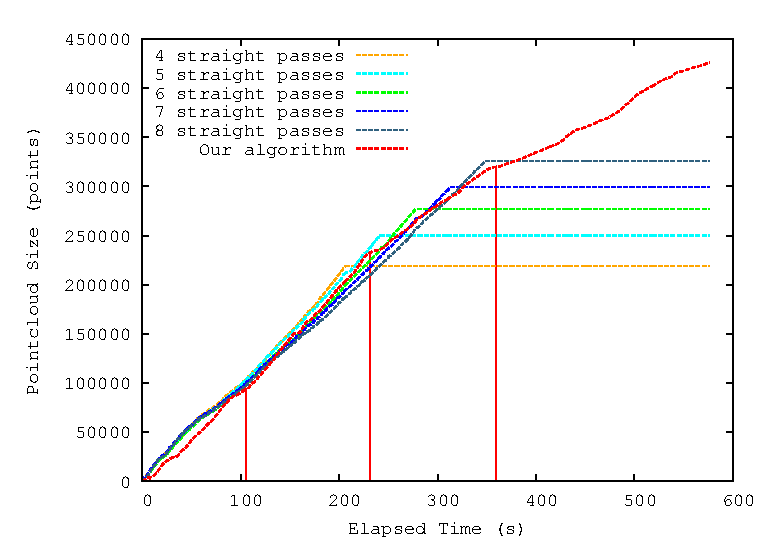
\includegraphics[width=0.48\textwidth]{images/graph_points_vs_time}
    \caption{Pointcloud size vs. flight-time using several waypoint generators. Vertical lines are drawn on every round of waypoint generation using our algorithm, executed after all previously generated waypoints have been passed.}
    \label{graph_points_vs_time}
\end{figure}

To assess our algorithms performance, we established the number of points stored in the pointcloud for a given flight-time as the primary metric. As explained in chapter \ref{complexity}, our octree-implementation allows setting a maximum point-density during construction. For the pointcloud storing the surface-reconstruction data, we defined the minimum distance between neighboring points to be $0.1m$. Because the number of points stored correlates directly to the scanned surface-area, measuring the number of points stored over time equals measuring the scanned surface area over time in meaning. All tests were executed in a simulator where the platform's angular velocity remained constant at $120 ^\circ/s$, while its linear velocity was limited to $2.8 m/s$ during all trials. After the scandata was streamed to the basestation using a TCP-connection, it was processed and statistics about flight-time and pointcloud sizes were logged.

The graph in Fig. \ref{graph_points_vs_time} shows results of using a simple, manually planned and collision-free scanline based exploration with trajectories similar to those for optimal complete terrain coverage in \cite{xu2011}. The results of scanning along these trajectories can be seen in Fig. \ref{cloud_top_scanlines_4} and \ref{cloud_top_scanlines_6} for four and six equidistant passes, respectively. As expected, flying more scanlines in the same area results in more points scanned, albeit with a visibly slower rate.

Additionally, the graph's red line depicts our algorithms' behavior: because the pointcloud needs an initial population for waypoint generation, the scanning rate stagnates shortly after launch during the first phase of waypoint generation, then reaches comparable speeds as the vehicle starts passing waypoints on the border between known and unknown environment. In this phase of flight, our algorithm is as efficient as a manually planned collision free optimal path, with the obvious advantage of having been generated automatically. Compared to exploring in scanline-fashion, the true strength in our method lies in the fact that on-line re-planning occurs such that when no more waypoints can be generated, gradually smaller sampling geometry is used to improve on ever smaller deficiencies in the reconstructed surface. This yields a truly dynamic and efficient scanning procedure that adapts well to many different kinds of outdoor scenarios.

\begin{figure}[htbp]
  \centering
  \subfigure[4 passes]{
    \label{cloud_top_scanlines_4}
    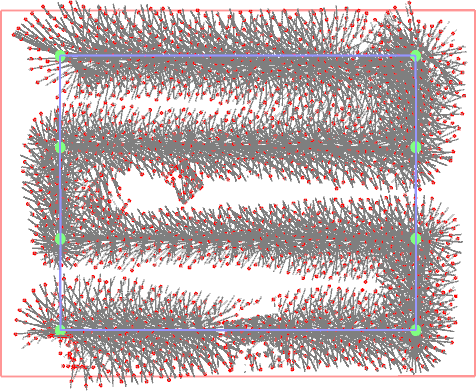
\includegraphics[width=0.22\textwidth]{images/cloud_top_scanlines_4} 
  }
  \subfigure[6 passes]{
    \label{cloud_top_scanlines_6}
    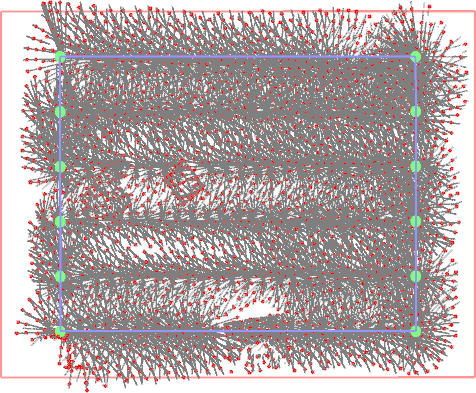
\includegraphics[width=0.22\textwidth]{images/cloud_top_scanlines_6} 
  }
  \caption{Pointclouds resulting from straight scanline passes. Note the unscanned surface in the bottom center shadowed by a roof.}
  \label{cloud_top_scanlines}
\end{figure}

\section{Outlook}

With the algorithm relying on collision detection between large numbers of static and dynamic objects, it is currently limited by the speed of collision detection. Physics-simulation in general and collision detection especially lend themselves well to optimization using massively-parallel implementations on GPUs. In the next steps, tests and extensions of the algorithm on GPUs are planned. Here, the questions of whether an increased number of sample geometry instances (up to a method that completely fills the user-defined scanning region with sample geometry) and their abidance over many iterations of the algorithm improves the waypoint generation is of special interest to the authors.

We plan to further extend our algorithm by adding another generation-mode for sampling geometry: when created along the bounding volume's top-plane, sample geometry is used to detect unscanned surfaces in all areas of the partially-reconstructed environment. A more efficient approach might also emit sampling geometry from the vehicle's current position with a velocity-vector matching the vehicle's course over ground. The authors expect that this would generate waypoints closer to the vehicle's position, requiring less distance to be travelled when visiting them. Also, as the age of computed waypoints grows, their associated information gain tends to decrease because the surfaces visible from their positions are often already scanned. Even worse, waypoints of older age are more susceptible to being enclosed by previously unscanned surface and thus unreachable. Although collision avoidance discards these waypoints in a later stage, not enqueueing them in the first place seems to be a better strategy.

% TODO shortened
%Finally, we plan to move our research's focus from waypoint generation to the problems of generating safely navigatable paths between them, dynamically replanning paths when necessary and discarding those that cannot be reached safely.

\begin{thebibliography}{99}

% ``Autonomous Exploration for 3D Map Learning'' by Johoo et al.

% Octrees
%\bibitem{meagher1982}
%Donald Meagher, Geometric modeling using octree encoding, {\it Computer Graphics and Image Processing}, 19, 2, pp. 129-147, (1982)

\bibitem{hota2009}
% 1mal
% Dubins Path, no wind
% viele referenzen auf airplanes mit wind uns dubins
Sikha Hota and Debasish Ghose, A Modified Dubins Method for Optimal Path Planning of a Miniature Air Vehicle Converging to a Straight Line Path, American Control Conference, St. Louis, MO, USA, 2009

\bibitem{mcneely2007}
% 1mal
% dubins vehicle und wind, wie kommeich am schnellsten von a nach b.
Rachelle L. McNeely and Ram V. Iyer and Phillip R. Chandler, Tour Planning for an Unmanned Air Vehicle under Wind Conditions, Journal of Guidance, Control, and Dynamics, Vol. 30, No. 5, September-October 2007

% 1 mal
\bibitem{chen2008}
Shengyong Chen and Y. F. Li and Jianwei Zhang and Wanliang Wang, Active Sensor Planning for Multiview Vision Tasks, Springer Verlag Berlin Heidelberg, 2008

\bibitem{mcgee2005}
% 1mal
Timothy G. McGee and Stephen Spry and J. Karl Hedrick, Optimal path planning in a constant wind with a bounded turning rate, Proc. of the AIAA Guidance, Navigation and Control Conference and Exhibit, San Francisco, CA, August 2005.

\bibitem{joho2007}
% 2mal
Dominik Joho and Cyrill Stachniss and Patrick Pfaff and Wolfram Burgard, Autonomous Exploration for 3{D} Map Learning, {\it {A}utonome {M}obile {S}ysteme {(AMS)}}, Springer, 2007, pp. 22-28

\bibitem{legrand2007}
% 2 mal
% macht broadphase per CUDA, gut erkl�rt in GPU gems 3, chapter 32
Scott Le Grand, Broad-Phase Collision Detection with CUDA, {\it GPU Gems 3, } (2007)

\bibitem{baraff1992}
% 1mal
David Baraff, Dynamic Simulation of Non-Penetrating Rigid Bodies, Cornell University, pp. 52 (1992)

\bibitem{gonzalez_banos2002}
% 1mal
% SLAM does not address the sensor-placement
% Extension to the ArtGallery-Problem
% Sensorkeulen von Kandidatenpunkten berechnen, 2D only
H\'{e}ctor H. Gonz\'{a}lez-Ba\~{n}os and Jean-Claude Latombe, Navigation Strategies for Exploring Indoor Environments, {\it I. J. Robotic Res.} 21(10-11), 829-848 (2002)

%\bibitem{haehnel2004}
% Pioneer und Sick zu Outdoor Modellen, 16seiten, kein Wort �ber next-best-view
%Dirk H\"ahnel and Wolfram Burgard and Sebastian Thrun, Learning Compact 3d Models of Indoor and Outdoor Environments with a Mobile Robot, {\it Elsevier Science Special Issue Eurobot} '01, 1-16

\bibitem{strand2009}
% 1mal
% Next-best-view centered. Occupancy grids are most common. cells are not binary, but carry probability.
% grid map mit ground, wall, unexplored
% ein gridcell ist dann guter next best view, wenn von ihm aus ein simulierter scan �ber m�glichst viele groundcells zu unexplored gebiet f�hrt.
% komische metrik, was spielts f�r ne rolle, wieivel ground der strahl passiert hat.
% das w�re in 3d zu teuer.
Marcus Strand and Ruediger Dillmann, Grid based next best view planning for an autonomous robot in indoor environments

%\bibitem{mikrokopterproject}
%Mikrokopter project, http://www.mikrokopter.de, 2011

%\bibitem{surmann2003}
% Indoor only, use ICP to fuse and localize robot.
% Next best View assumes free sensor orientation. Not possible with driving robots, but possible with mikrokopter.
% Next best View is Art Gallery problem: Where to place guards so that they see everything.
%  J. O?Rourke, Art Gallery Theorems and Algorithms, OxfordUniversity, Oxford, 1987
% Man scannt, baut dann eien Grundriss und verbindet bekannte linien mit unbekannten linien. Die unbekannte Linie, die die meisten �berschenidungen mit laserscannerlinien hat, wird als n�chstes gescannt -> highest information gain.
% Suppose a 2D map of an art gallery is given by a polygon P, having n corners (vertices) and n walls (lines). If a watchman sees everything that lies on a straight line from his position, then the maximal number of guards needed is n/3 [27]. Finding the minimum number of watchmen needed for this task is NP hard, since it can be reduced to the 3-SAT problem [27]. Gonzalez-Banos et al. reduce the art gallery problem to set cover and approximate the latter one. Set cover is de?ned as follows: given a pair (X, F), where X is some ?nite set. F is a subset of the power set of X, i.e., (F ? P(X)) and X = s?F s. Find the C ? F , such that X = s?C C and the set C has a minimum number of elements.
%Hartmut Surmann and Andreas Nuechter and Joachim Hertzberg, An autonomous mobile robot with a 3D laser range finder for 3D exploration and digitalization of indoor environments, Robotics and Autonomous Systems 45 (2003) pp. 181-198

\bibitem{walthelm2011}
% 2mal
% 2d occupancy map (float)
% Man blickt in regionen, f�r die noch keine oder nur unsichere belegungshypothesen bekannt sind.
% und dann f�hrt man wohl an einen punkt, von dem m�glichst viele dieser regionen sichtbar sind.
Axel Walthelm and Amir Madany Mamlouk, Multisensoric Active Spatial Environment Exploration and Modeling (2011)

\bibitem{yamauchi1998}
% 2mal
% 2d only
% The central question in exploration is: Given what you know about the world, where should you move to gain as much new information as possible?
% es gibt ein 2d grid, in dem die occupancy probability gespeichert wird.
% dann einfach edge detection und schon hat man die frontiers.
Brian Yamauchi, Frontier-Based Exploration Using Multiple Robots, Proceedings of the Second International Conference on Autonomous Agents, Minneanapolis, ACM Press, 1998

\bibitem{shade2011}
% 2mal
% occupancy grid and exploration boundaries, map besteht aus voxeln.
Robbie Shade and Paul Newman, Choosing Where To Go: Complete 3D Exploration With Stereo, IEEE International Conference on Robotics and Automation, 2011

\bibitem{orourke1987}
% 1mal
Joseph O'Rourke, Art Gallery Theorems and Algorithms, Oxford University Press, Oxford, 1987

%\bibitem{shen2011}
% Fliegen mit Asctec durch Innenr�ume, IMU und LIDAR geben Pose
% Gutes SLAM, aber nur 2D auf mehreren Floors
%Shaojie Shen and Nathan Michael and Vijay Kumar, Autonomous Multi-Floor Indoor Navigation with a Computationally Constrained MAV, IEEE International Conference on Robotics and Automation, 2011

\bibitem{triebel2006}
% 1mal
%Rudolph Triebel and Patrick Pfaff and Wolfram Burgard, Multi-Level Surface Maps for Outdoor Terrain Mapping and Loop Closing, Proceedings of the 2006 IEEE/RSJ International Conference on Intelligent Robots and Systems 2006
Rudolph Triebel et al., Multi-Level Surface Maps for Outdoor Terrain Mapping and Loop Closing, Proceedings of the 2006 IEEE/RSJ IROS 2006

%\bibitem{andert2011}
% 0mal
% Obstacle avoidance, path re-planning mit benzin-hubschrauber am DLR
% Cool, aber obstacle avoidance ist noch nciht mein thema?!
%Franz Andert and Florian Adolf and Lukas Goormann and Joerg Dittrich, Mapping and Path Planning in Complex Environments: An Obstacle Avoidance Approach for an Unmanned Helicopter, IEEE International Conference on Robotics and Automation, 2011

%\bibitem{strand2008}
% 0mal
%Marcus Strand and Ruediger Dillmann, Using an attributed 2D-grid for next-best-view planning on 3D environment data for an autonomous robot

\bibitem{xu2011}
% 1mal
% Generieren sich optimale pfade, scanline-�hnlich mit holonomem uav, fixed wing.
Anqi Xu and Chatavut Viriyasuthee and Ioannis Rekleitis, Optimal Complete Terrain Coverage Using an Unmanned Aerial Vehicle, IEEE International Conference on Robotics and Automation, 2011

%\bibitem{sun2002}
% 1mal, unwichtig
% machen 3d reconstruction und sind stolz auf watertightness.
%Y. Sun and J. K. Paik and A. Koschan and M. A. Abidi, 3D Reconstruction of Indoor and Outdoor Scenes Using a Mobile Range Scanner

\bibitem{sormann2007}
% 1mal
% watertight reconstruction
Mario Sormann and Christopher Zach and Joachim Bauer and Konrad Karner and Horst Bishof, Watertight Multi-view Reconstruction Based on Volumetric Graph-Cuts

\bibitem{hornung2006}
% 1mal
% watertight reconstruction
Alexander Hornung and Leif Kobbelt, Robust Reconstruction of Watertight 3D Models from Non-uniformly Sampled Point Clouds Without Normal Information

\end{thebibliography}

\end{document}

